%!TEX root = ../main.tex
\section{Αρχιτεκτονική των FPGA}

Μια γενική άποψη ενός \gls{fpga} board αποκαλύπτει αρκετά ηλεκτρονικά εξαρτήματα που συνεργάζονται για να υλοποιήσουν τα επιθυμητά ψηφιακά κυκλώματα. Η κύρια λειτουργική μονάδα ενός \gls{fpga} είναι το \gls{clb}. Αυτά είναι οι κύριοι λογικοί πόροι που επιτρέπουν την υλοποίηση ακολουθιακών αλλά και συνδυαστικών κυκλωμάτων. Κάθε πλακέτα περιλαμβάνει έναν μεγάλο αριθμό \gls{clb}, τα οποία οργανώνονται σε μία διδιάστατη διάταξη συνδεδεμένη μέσω οριζόντιων και κάθετων καναλιών.
\begin{figure}[H]
  	\centering
	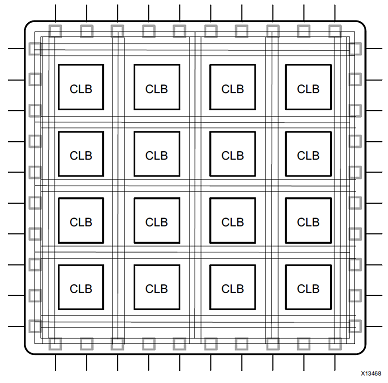
\includegraphics[width=0.45\textwidth]{images/basic_fpga}\\
	\caption{Βασική αρχιτεκτονική FPGA\cite{clb1}}
	\label{fig:basic_fpga}
\end{figure}

Υπάρχουν επίσης αρκετά I/O blocks που επιτρέπουν στην συσκευή να επικοινωνεί με το περιβάλλον.

Κάθε \gls{clb} αποτελείται από slices, καθένα από τα οποία περιλαμβάνει κάποιον αριθμό λογικών κελιών. O αριθμός αυτός εξαρτάται από το εκάστοτε μοντέλο FPGΑ και κατά συνέπεια τον κατασκευαστή του. Κάθε λογικό κελί αποτελείται από τα ακόλουθα:
\begin{itemize}
\item \gls{lut} - Το στοιχείο αυτό πραγματοποιεί λογικές πράξεις.
\item Flip-Flop (FF) - Είναι καταχωρητές που αποθηκεύουν τα αποτελέσματα των \gls{lut}s.
\item Διασυνδέσεις (καλώδια)
\item Input/Output (I/O) pads - Είναι φυσικές πύλες για τη μεταφορά δεδομένων από/προς το \gls{fpga}.\\
\end{itemize}

Παρ' όλο που η δομή αυτή επαρκεί για την υλοποίηση οποιουδήποτε αλγορίθμου, η αποδοτικότητα της υλοποίησης είναι περιορισμένη από άποψη υπολoγιστικού \gls{throughput}, απαιτούμενων πόρων καθώς και συχνότητας του ρολογιού. Για το λόγο αυτό, οι σύγχρονες αρχιτεκτονικές \gls{fpga} ενσωματώνουν τα βασικά στοιχεία μαζί με επιπλέον υπολογιστικά και blocks αποοθήκευσης μνήμης που αυξάνουν την υπολογιστική ισχύ καθώς και την απόδοση της. Τα στοιχεία αυτά, τα οποία αναλύονται στην επόμενη ενότητα, είναι:
\begin{itemize}
\item Ενσωματωμένες μνήμες για κατανεμημένη αποθήκευση δεδομένων
\item \gls{pll} για την επίτευξη διαφορετικών συχνοτήτων ρολογιού του \gls{fpga} fabric
\item Σειριακοί πομποδέκτες υψηλής ταχύτητας
\item Ελεγκτές μνήμης εκτός του chip
\item Multiply-accumulate blocks \\
\end{itemize}

Ο συνδυασμός όλων των \gls{clb}s είναι υπεύθυνος για την υλοποίηση οποιασδήποτε εφαρμογής. Υπεύθυνα όμως για την πραγματοποίηση πολλαπλών σχεδίων είναι τα `switch matrices', που διαμορφώνονται κάθε φορά ανάλογα με το σχέδιο που υλοποείται. Μια λεπτομερέστερη άποψη των \gls{clb} και των switch matrices φαίνεται στο ακόλουθο σχήμα:
\begin{figure}[H]
  	\centering
	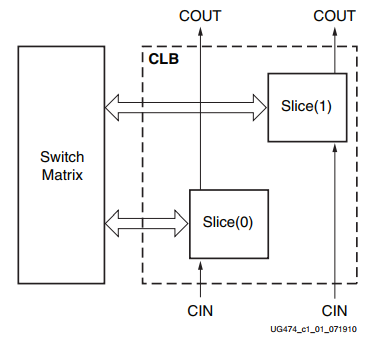
\includegraphics[width=0.4\textwidth]{images/clb}\\
	\caption{Δομή \gls{clb} \cite{clb}}
\end{figure}
\subsection{LUT}

Το \gls{lut} είναι το βασικό κατασκευαστικό block των \gls{fpga} και είναι ικανό να υλοποιεί οποιαδήποτε λογική συνάρτηση $N$ boolean μεταβλητών. Βασικά, το στοιχείο αυτό αποτελεί έναν πίνακα αληθείας όπου διάφοροι συνδυασμοί των εισόδων υλοποιούν διαφορετικές πράξεις και παράγουν αντίστοιχα αποτελέσματα στην έξοδο τους. Καθώς το όριο των εισόδων στον πίνακα αληθείας είναι $N$, οι μέγιστες τιμές εξόδου που μπορεί να υπολογίσει το \gls{lut} είναι $2^N$, που αντιστοιχούν στις θέσεις μνήμης που μπορεί να προσπελάσει. Τυπική τιμή του $N$ για τα FGPA της Xilinx είναι 6.
\begin{figure}[H]
  	\centering
	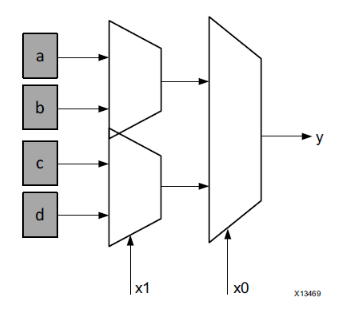
\includegraphics[width=0.6\textwidth]{images/lut}\\
	\caption{Δομή LUT \cite{lut}}
\end{figure}

Η υλοποίηση στο υλικό ενός \gls{lut} μπορεί να θεωρηθεί σα μία συλλογή από κελιά μνήμης συνδεδεμένα σε ζευγάρια πολυπλεκτών. Οι είσοδοι των \gls{lut} δρουν σαν selector bits του πολυπλέκτη ο οποίος επιλέγει το αποτέλεσμα σε κάθε δεδομένη χρονική στιγμή. Είναι πολύ σημαντικό να έχουμε στο νου μας αυτή την αναπαράσταση καθώς ένα \gls{lut} μπορεί να χρησιμοποιηθεί τόσο για τον υπολογισμό κάποιας συνάρτηση όσο και ως στοιχείο μνήμης.
\subsection{Flip Flops}

Η βασική δομή ενός Flip-Flop περιλαμβάνει μία είσοδο δεδομένων, έναν παλμό ρολογιού, ένα σήμα reset και μία έξοδο δεδομένων. Κατά την κανονική λειτουργία του, οποιαδήποτε τιμή στην είσοδο του είναι μανδαλωμένη και μεταφέρεται στην έξοδο σε κάθε παλμό του ρολογιού. Ο σκοπός του clock enable pin είναι να επιτρέπει στο Flip-Flop να διατηρεί μια συγκεκριμένη τιμή για περισσότερους από έναν παλμούς ρολογιού. Νέα δεδομένα στην είσοδο απλώς μανδαλώνονται και περνούν στην έξοδο μόνο όταν το ρολόι αλλά και το clock enable είναι ίσα με 1.
\begin{figure}[H]
  	\centering
	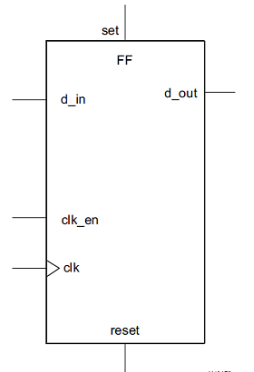
\includegraphics[width=0.3\textwidth]{images/FF}\\
	\caption{Flip-Flop \cite{ff}}
\end{figure}
\subsection{DSP48}

Τα \gls{fpga} είναι αποδοτικά στην εκτέλεση εφαρμογών \gls{dsp} καθώς μπορούν να υλοποιήσουν κατά-παρραγελία, πλήρως παραλληλοποιημένους αλγορίθμους. Οι εφαρμογές \gls{dsp} χρησιμοποιούν πολλούς δυαδικούς πολλαπλασιαστές και συσσωρευτές οι οποίοι είναι καλύτερα υλοποιήσιμοι στα \gls{dsp} Slices. Όλα τα σύγχρονα \gls{fpga} της Xilinx διαθέτουν πολλά αποκλειστικά, πλήρως διαμορφώσιμα και χαμηλής κατανάλωσης \gls{dsp} Slices τα οποία συνδυάζουν υψηλή ταχύτητα με μικρό μέγεθος ενώ διατηρούν την ευελιξία του σχεδιασμού του συστήματος σε υψηλό επίπεδο. Τα \gls{dsp} Slices ενισχύουν την ταχύτητα και την απόδοση πολλών εφαρμογών πέρα από την σκοπιά της Ψηφιακής Επεξεργασίας Σημάτων, όπως για παράδειγμα σε wide dynamic bus shifters, memory address generators, wide bus multiplexers και memory-mapped I/O registers. Η βασική λειτουργικότητα των DSP48 slices φαίνεται στο ακόλουθο σχήμα.
\begin{figure}[H]
  	\centering
	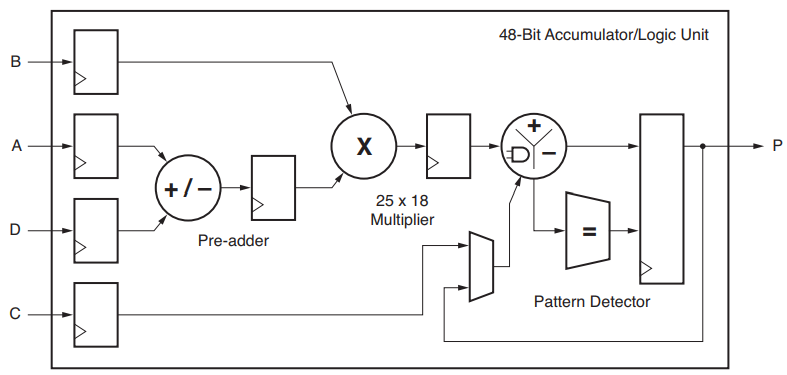
\includegraphics[width=0.65\textwidth]{images/dsp48}
	\caption{DSP48 Slice \cite{DSP48}}
	\label{fig:DSP48}
\end{figure}
\hyphenation{re-quire-ments}
Μερικά χαρακτηριστικά της λειτουργικότητας των DSP Slices είναι:
\begin{itemize}
	\item 25x18 πολλαπλασιαστές συμπληρώματος ως προς 2:
	\subitem Dynamic bypass
	\item Συσσωρευτής 48bit:
	\subitem Μπορεί να χρησιμοποιηθεί σαν ασύγχρονος απαριθμητής
	\item Pre-adder χαμηλής κατανάλωσης:
	\subitem Βελτιστοποιεί εφαρμογές συμμετρικών φίλτρων και μειώνει την κατανάλωση των DSP Slices
	\item Single-instruction-multiple-data (SIMD) αριθμητική μονάδα:
	\subitem Dual 24-bit ή quad 12-bit add/subtract/accumulate
	\item Προαιρετική λογική μονάδα:
	\subitem Μπορεί να παράξει οποιαδήποτε από τις δέλα λογικές πράξεις δύο τελεστών
	\item Ανιχνευτής προτύπων
	\item Προχωρημένα χαρακτηριστικά:
	\subitem Προαιρετικό pipelining
\end{itemize}
\subsection{BRAM \& Άλλες μνήμες}

Το \gls{fpga} Fabric περιλαμβάνει ενσωματωμένα στοιχεία μνήμης τα οποία μπορούν να χρησιμοποιηθούν ως μνήμες RAM, ROM ή καταχωρητές ολίσθησης. Τα στοιχεία αυτά είναι block RAMs (BRAMs), \gls{lut} και καταχωρητές ολίσθησης αντίστοιχα.

Τo BRAM είναι ένα στοιχείο RAM δύο θυρών ενσωματωμένο στο \gls{fpga} fabric για να παρέχει αποθηκευτικό χώρο για μεγάλο αριθμό δεδομένων. Οι δύο τύποι BRAM που είναι διαθέσιμοι σε μια συσκευή μπορούν να αποθηκεύσουν είτε 18k είτε 36k bits και το σύνολο του αποθηκευτικού χώρου διαφέρει με την συσκευή. Λόγω των δύο θυρών που διαθέτουν, επιτρέπεται η παράλληλη και στον ίδιο παλμό ρολογιού πρόσβαση δεδομένων σε διαφορετικές θέσεις.
\begin{figure}[ht]
  	\centering
	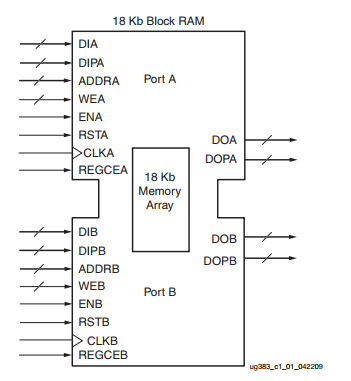
\includegraphics[width=0.35\textwidth]{images/bram}\\
	\caption{Dual Port BRAM \cite{bram}}
\end{figure}

Όπως αναφέρθηκε και προηγουμένως, το \gls{lut} είναι μια μικρή μνήμη στην οποία εγγράφονται τα περιεχόμενα ενός πίνακα αληθείας. Λόγω της ευελιξίας των \gls{lut} στα \gls{fpga} της Xilinx, τα blocks αυτά μπορούν να χρησιμοποιηθούν και ως 64bit μνήμες και αναφέρονται συνήθως σαν κατανεμημένη μνήμη. Είναι ο πιο γρήγορος διαθέσιμος τύπος μνήμης στα \gls{fpga}, καθώς μπορεί να ενσωματωθεί σε οποιοδήποτε σημείο του fabric που βελτιώνει την απόδοση του κυκλώματος προς υλοποίηση.

Ο shift register (καταχωρητής ολίσθησης) μπορεί να θεωρηθεί ως μία αλυσίδα καταχωρητών συνδεδεμένων ο ένας με τον άλλον. Ο σκοπός της δομής αυτής είναι να παρέχει τη δυνατότητα της επαναχρησιμοποίησης των δεδομένων κατά μήκος ενός υπολογιστικού μονοπατιού, π.χ. κατά την κατασκευή ενός φίλτρου. Για παράδειγμα, ένα βασικό φίλτρο αποτελείται από μια σειρά πολλαπλασιαστών που πολλαπλασιάζουν ένα δείγμα δεδομένων με ένα σετ συντελεστών. Χρησιμοποιώντας έναν shift register για την αποθήκευση των δεδομένων εισόδου, μία ενσωματωμένη δομή μεταφοράς μεταφέρει τα δείγματα στον επόμενο πολλαπλασιαστή στην αλυσίδα σε κάθε παλμό του ρολογιού.
\begin{figure}[H]
  	\centering
	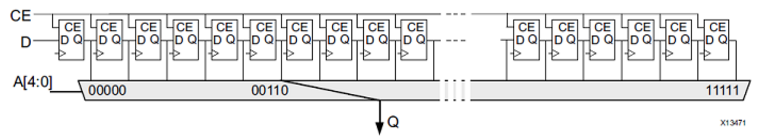
\includegraphics[width=0.75\textwidth]{images/shftreg}\\
	\caption{Addressable Shift Register \cite{bram}}
\end{figure}
\section{Zynq-7000 ApSoc}

Η οικογένεια Zynq®-7000 της Xilinx είναι βασισμένη στην αρχιτεκτονική `Xilinx All Programmable SoC'. Τα προϊόντα αυτά περιέχουν έναν διπύρηνο ή μονοπύρηνο ARM® Cortex™-A9 που αποτελεί το \gls{ps} και την \gls{pl} κατασκευασμένη στα 28nm. H ARM Cortex-A9 CPU είναι το κέντρο του \gls{ps} και περιλαμβάνει επίσης on-chip μνήμη, εξωτερικές διασυνδέσεις μνήμης και ένα πλούσιο σετ απο διεπαφές περιφερειακών. Όλα αυτά καθιστούν την οικογένεια Zynq®-7000 να διαθέτει πολύ γρήγορη αλληλεπίδραση κατά τη διάρκεια επιτάχυνσης εφαρμογών. \cite{ds190}

Η οικογένεια Zynq-7000 προσφέρει την ευελιξία και την επεκτασιμότητα ενός \gls{fpga}, παρέχοντας παράλληλα απόδοση, ισχύ και ευκολία χρήσης που συσχετίζεται συνήθως με \gls{asic} και \gls{assp}s. Το φάσμα των συσκευών της οικογένειας Zynq-7000 επιτρέπει στους σχεδιαστές να στοχεύσουν ευαίσθητες ως προς το κόστος καθώς και εφαρμογές υψηλής απόδοσης από μια ενιαία πλατφόρμα χρησιμοποιώντας εργαλεία που βασίζονται σε βιομηχανικά πρότυπα. Ενώ κάθε συσκευή της οικογένειας Zynq-7000 περιέχει το ίδιο \gls{ps}, οι πόροι των \gls{pl} και I/O  διαφέρουν μεταξύ των συσκευών. Ως αποτέλεσμα, τα Zynq-7000S SoCs είναι σε θέση να εξυπηρετούν ένα ευρύ φάσμα εφαρμογών, όπως: \\

\begin{itemize}
	\item Βοήθεια οδηγού, πληροφορίες και ψυχαγωγία
	\item Κάμερα εκπομπής
	\item Έλεγχος βιομηχανικού κινητήρα, βιομηχανική δικτύωση και μηχανική όραση
	\item IP και έξυπνη κάμερα
	\item LTE radio και baseband
	\item Ιατρική διάγνωση και απεικόνιση
	\item Εξοπλισμός βίντεο και νυχτερινή όραση \\
\end{itemize}

Η αρχιτεκτονική Zynq-7000 επιτρέπει την υλοποίηση προσαρμοσμένης λογικής στο \gls{pl} και προσαρμοσμένο λογισμικό στο \gls{ps} για την πραγματοποίηση μοναδικών και διαφοροποιημένων λειτουργιών του συστήματος. Η ενσωμάτωση του \gls{ps} με το \gls{pl} επιτρέπει επίπεδα απόδοσης που δε μπορούν να επιτευχθούν από ένα σύστημα 2 chips (πχ ένα ASSP με ένα \gls{fpga}) λόγω της περιορισμένης εύρους ζώνης I/O, της καθυστέρησης παραγωγής δεδομένων και του προϋπολογισμού ισχύος.

Η Xilinx προσφέρει ένα μεγάλο αριθμό IPs για την οικογένεια Zynq-7000. Προγράμματα οδήγησης συσκευών τόσο αυτόνομα όσο και για Linux είναι διαθέσιμα για τα περιφερειακά του \gls{ps} και του \gls{pl}. Το περιβάλλον ανάπτυξης Vivado® Design Suite επιτρέπει γρήγορη ανάπτυξη προϊόντων. Η υιοθέτηση του βασισμένου σε ARM υπολογιστικού συστήματος συνδυάζει ένα ευρύ φάσμα εργαλείων τρίτων με το υπάρχον οικοσύστημα \gls{pl} της Xilinx. Η συμπερίληψη ενός επεξεργαστή εφαρμογών επιτρέπει την υποστήριξη υψηλού επιπέδου λειτουργικών συστημάτων, όπως το Linux. Άλλα τυπικά λειτουργικά συστήματα που χρησιμοποιούνται με τον επεξεργαστή Cortex-A9 είναι επίσης διαθέσιμα για την οικογένεια Zynq-7000.

Το \gls{ps} και το \gls{pl} βρίσκονται σε χωριστούς τομείς ισχύος, επιτρέποντας στον χρήστη αυτών των συσκευών να απενεργοποιήσουν την \gls{pl} εάν απαιτείται για να επιτύχουν καλύτερη διαχείριση ισχύος. Οι επεξεργαστές στο \gls{ps} πάντα εκκινούν πρώτα, επιτρέποντας μια εστιασμένη στο λογισμικό προσέγγιση για τη διαμόρφωση του \gls{pl}. Τη διαμόρφωση \gls{pl} διαχειρίζεται λογισμικό που εκτελείται στη CPU.

Η οικογένεια Zynq-7000 της Xilinx περιλαμβάνει ένα μεγάλο αριθμό συσκευών με διαφορετικό αριθμό πόρων. Μπορούμε να τις διαχωρίσουμε σε δύο υποκατηγορίες: Cost-optimized και- Mid-Range. Στο ακόλουθο σχήμα φαίνονται οι συσκευές και τα χαρακτηριστικά τους. \cite{Crockett:2014:ZBE:2685817}

\begin{figure}[H]
  	\centering
	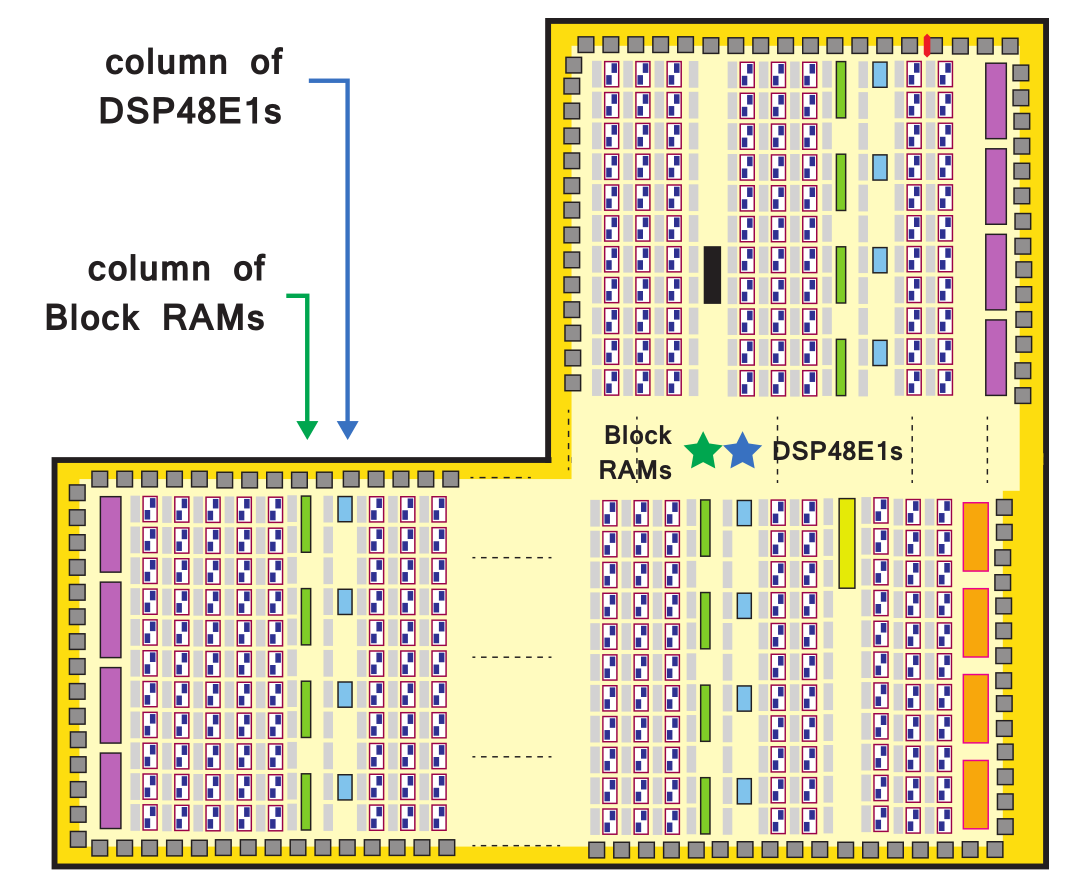
\includegraphics[width=0.75\textwidth]{fabric}\\
	\caption{Programming Logic \cite{Crockett:2014:ZBE:2685817}}
\end{figure}
% https://www.xilinx.com/support/documentation/selection-guides/zynq-7000-product-selection-guide.pdf
\begin{figure}[H]{}
  	\centering
	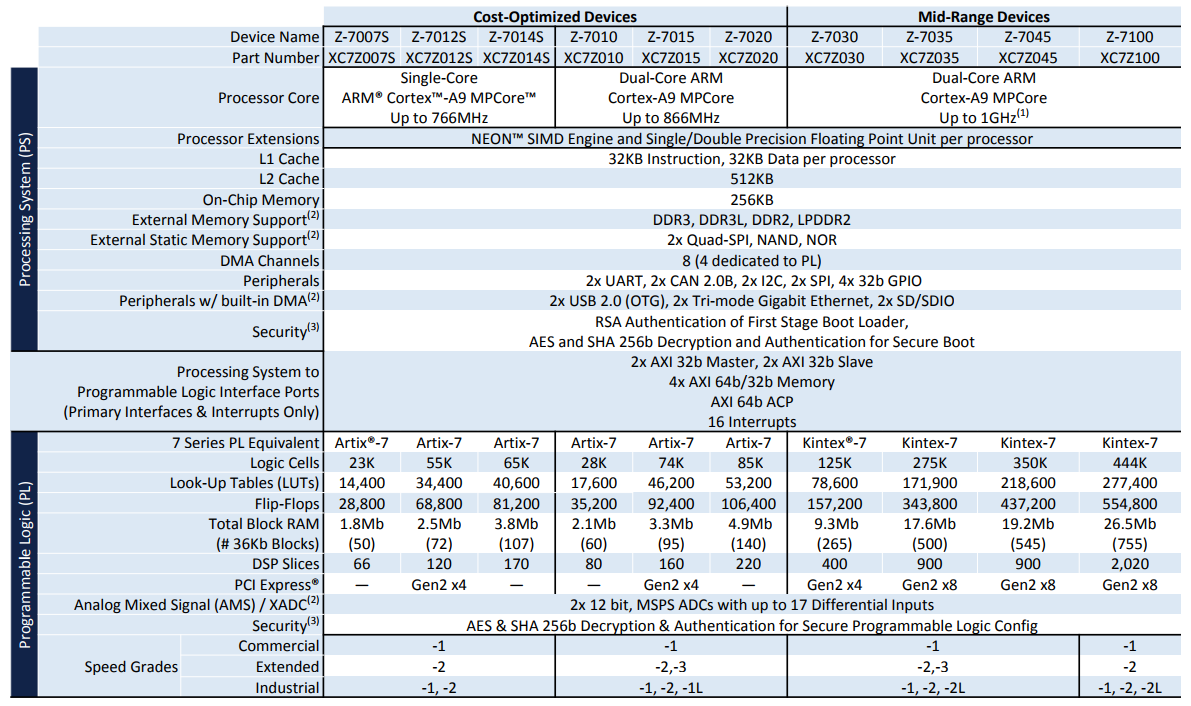
\includegraphics[width=\textwidth]{devices}\\
	\caption{Zynq®-7000 All Programmable SoC Family \cite{Zynq700083:online}}
\end{figure}

\subsection{Application Processing Unit (APU)}

To \gls{ps} του Zynq εκτός από τους πυρήνες ARM περιλαμβάνει και ένα set υπολογιστικών πόρων, σχηματίζοντας έτσι ένα \gls{apu}, το οποίο φαίνεται στο ακόλουθο σχήμα.

Το \gls{apu} αποτελείται κυρίως από τους δύο ARM πυρήνες, καθένας από τους οποίους περιλαμβάνει: έναν NEON Media Processing Engine και Floating Point Unit, μία Memory Management Unit καθώς και μνήμες cache. Τέλος, η μονάδα Snoop Control δημιουργεί μία διασύνδεση μεταξύ των ARM, των μνημών και του \gls{pl}. Η SCU διαχειρίζεται όλες τις συναλλαγές μεταξύ των \gls{ps} και \gls{pl} μέσω της \gls{acp}.
\begin{figure}[H]{}
  	\centering
	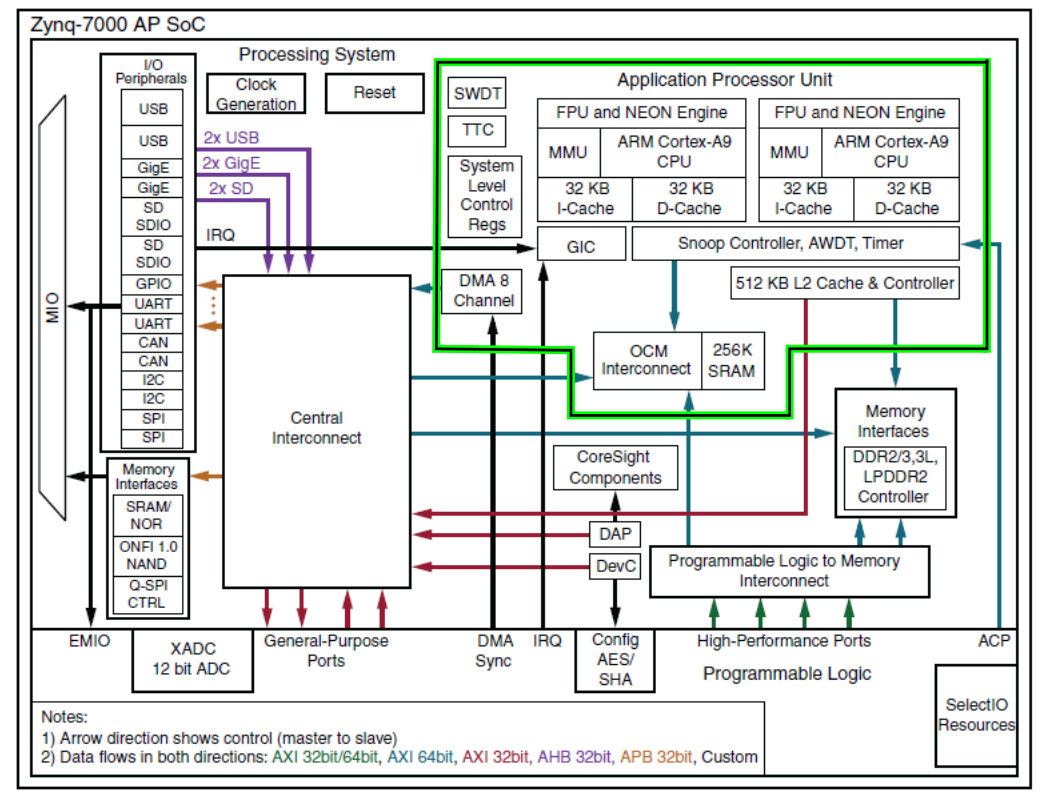
\includegraphics[width=0.7\textwidth]{apu}\\
	\caption{Zynq APU \cite{Crockett:2014:ZBE:2685817}}
\end{figure}
\begin{figure}[H]{}
  	\centering
	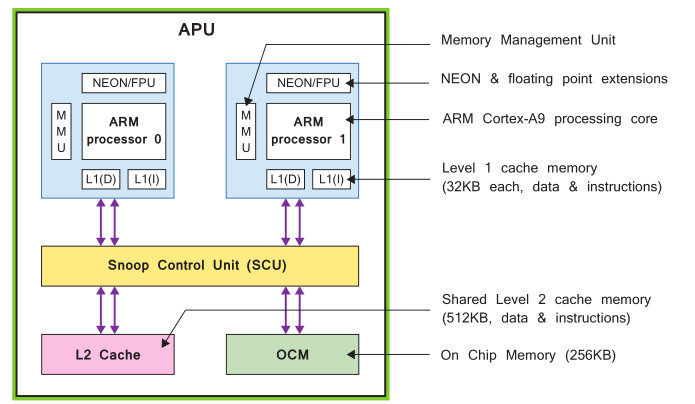
\includegraphics[width=0.6\textwidth]{apublock}\\
	\caption{APU Block diagram \cite{Crockett:2014:ZBE:2685817}}
\end{figure}

\section{ZC702 Evaluation Kit}
Η συσκευή που χρησιμοποιήθηκε στην παρούσα διπλωματική είναι το ZC702 Evaluation Kit της Xilinx που περιλαμβάνει το Zynq-7000 XC7Z020-1CLG484C \gls{apsoc} και είναι αντίστοιχο με ένα Artix-7 \gls{fpga}. Ανήκει στο low-end κομμάτι των προϊόντων της αρχιτεκτονικής Zynq-7000 με 85K9 Logic Cells, 53.200 \gls{lut}, 106.400 Flip-Flops και 220 \gls{dsp} slices με 560KB BRAM. To ZC702 evaluation board παρέχει ένα περιβάλλον υλικού για την ανάπτυξη και την αξιολόγηση σχεδίων. Το \gls{ps} περιλαμβάνει δύο πυρήνες ARM® Cortex™-A9 MPCore™, διασύνδεση AMBA®, εσωτερική μνήμη, εξωτερικές διεπαφές μνήμης καθώς και περιφερειακά όπως: USB, Ethernet, SPI, SD/SDIO, I2C, CAN, \gls{uart} και GPIO. Στο \ref{fig:zc702board} φαίνεται το board ανάπτυξης ZC702. Τα κυριότερα χαρακτηριστικά του είναι:
\begin{itemize}
	\item Zynq XC7Z020-1CLG484C
	\item 1 GB DDR3
	\item 128 Mb Quad SPI flash memory
	\item USB 2.0 ULPI
	\item Secure Digital (SD) connector
	\item USB JTAG
	\item USB-to-\gls{uart}
	\item HDMI codec
	\item I$^2$C
	\item Status LEDs
	\item User I/O
	\item VITA 57.1 FMC LPC connectors
	\item Dual 12-bit 1 MS\gls{ps} XADC analog-to-digital front end \\
\end{itemize}
\begin{figure}[H]
  	\centering
	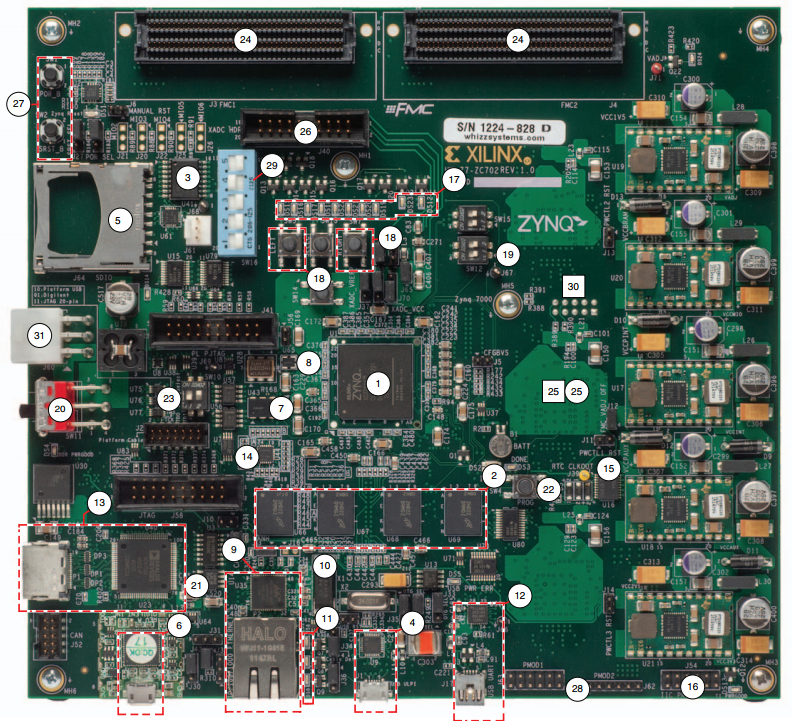
\includegraphics[width=0.7\textwidth]{zc702board}
	\caption{ZC702 Evaluation kit \cite{UG926}}
	\label{fig:zc702board}
\end{figure}

Στο σχήμα \ref{fig:hlbd} φαίνεται το λογικό διάγραμμα υψηλού επιπέδου με τις διασυνδέσεις του υπολογιστικού συστήματος με την \gls{pl}. \\

\begin{figure}[H]
  	\centering
	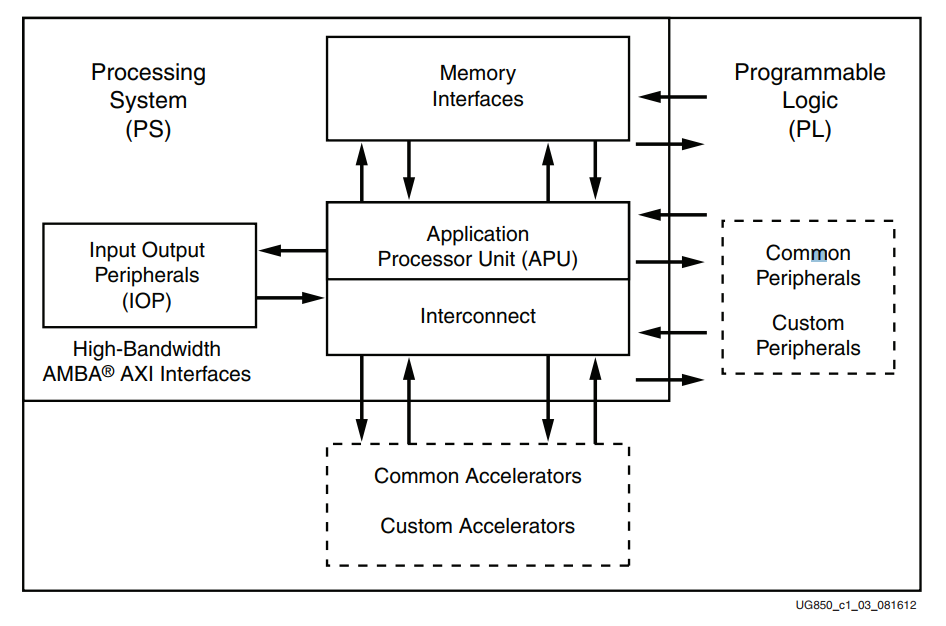
\includegraphics[width=0.8\textwidth]{zc702}\\
	\caption{Λογικό διάγραμμα υψηλού επιπέδου \cite{ug850}}
	\label{fig:hlbd}
\end{figure}

\newpage Στη συνέχεια θα γίνει αναφορά στις διάφορες συσκευές και περιφερειακά που χρησιμοποιήθηκαν στην παρούσα εργασία.

\subsection{Διαμόρφωση συσκευής}

Η συσκευή χρησιμοποιεί μια διαδικασία εκκίνησης πολλαπλών σταδίων που υποστηρίζει τόσο ασφαλή όσο και μη ασφαλή εκκίνηση. Το υπολογιστικό σύστημα είναι ο κύριος της διαδικασίας εκκίνησης και διαμόρφωσης. Για ασφαλή εκκίνηση, το \gls{pl} πρέπει να είναι ενεργοποιημένο για να επιτρέψει τη χρήση του του μπλοκ ασφαλείας το οποίο παρέχει αποκρυπτογράφηση/πιστοποίηση ταυτότητας 256 bit AES \& SHA. Οι επιλογές διαμόρφωσης είναι οι ακόλουθες:
\begin{itemize}
	\item Ρύθμιση \gls{ps}: Μνήμη flash Quad SPI
	\item Διαμόρφωση \gls{ps}: Εκκίνηση συστήματος επεξεργαστή από κάρτα SD ή μέσω SDK
	\item Διαμόρφωση \gls{pl}: Θύρα διαμόρφωσης USB JTAG ή Platform cable JTAG
\end{itemize}
\subsection{USB-to-UART Bridge}

Η πλακέτα ZC702 περιέχει μια USB-to-\gls{uart} συσκευή της Silicon Labs (CP2103GM) που επιτρέπει τη σύνδεση με έναν κεντρικό υπολογιστή μέσω θύρας USB. Οι ακροδέκτες του - TX \& RX - είναι συνδεδεμένοι στο μπλοκ IP του \gls{uart}\_1 που βρίσκεται εντός των περιφερειακών του XC7Z020 \gls{apsoc}.
\subsection{AXI4}

To ΑΧΙ είναι κομμάτι του ARM AMBA, μίας οικογένεις μικροελεγκτών και διασυνδέσεων που έκανε την εμφάνισή της το 1996. Η τελευταία έκδοση κυκλοφόρησε το 2010 και περιλαμβάνει τη δεύερη έκδοση του AXI, AXI4. Υπάρχουν 3 τύποι διεπαφών AXI4:
\begin{itemize}[leftmargin=*]
	\item{AXI4 - high-performance memory-mapped requirements}
	\item{AXI4-Lite - simple, low-throughput memory-mapped communication}
	\item{AXI4-Stream - high-speed streaming data}
\end{itemize}

Στην εργασία για τη μεταφορά δεδομένων, θα χρησιμοποιηθεί κυρίως το AXI4-Stream με τo S\_AXI\_HP το οποίο είναι μία διεπαφή υψηλής απόδοσης ανάμεσα στο \gls{pl} και το \gls{ps}. Επιτρέπει ένα κανάλι μεγάλου throughput και αποτελεί έναν από του βέλτιστους τρόπους μεταφοράς μεγάλων όγκων δεδομένων σε εφαρμογές video, υλοποίησης φίλτρων κά.
\section{Software}
\subsection{Εισαγωγή}

Ανάλογα με την απόδοση και την ευκολία προγραμματισμού του συστήματος, ο μηχανικός είναι επιφορτισμένος με τον καθορισμό της καλύτερης πλατφόρμας υλοποίησης ώστε να βγάλει το προϊόν στην αγορά. Για να φέρει το έργο του εις πέρας, έχει τη βοήθεια των διάφορων τεχνικών προγραμματισμού και μιας ποικιλίας πλατφορμών επεξεργασίας υλικού.

Στον τομέα του προγραμματισμού, τις τελευταίες δεκαετίες έχουν γίνει σημαντικές βελτιώσεις στον αντικειμενοστραφή προγραμματισμό και στην παράλληλη επεξεργασία ώστε να επιτευχθεί αύξηση της απόδοσης. Οι πρόοδοι στις γλώσσες προγραμματισμού επέτρεψαν στο μηχανικό να δημιουργεί και να δοκιμάζει προσεγγίσεις με πολύ γρήγορο ρυθμό. Η ανάγκη όμως αυτή, για γρήγορη ανάπτυξη συστημάτων οδήγησε στο ερώτημα του που θα εκτελείται ο αλγόριθμος.

Σχετικά με την πλατφόρμα στην οποία θα εκτελείται ο αλγόριθμος, υπάρχουν αρκετές επιλογές για έναν μηχανικό, όπως για παράδειγμα \gls{asic}, \gls{fpga}, \gls{mpsoc}. Τονίζουμε ότι υπάρχει μια συνεχώς αυξανόμενη εστίαση στην παραλληλοποίηση και ταυτόχρονη εκτέλεση εντολών.

Έχουν γίνει σημαντικές πρόοδοι στην κατασκευή των \gls{asic} βελτιώνοντας κατά πολύ την απόδοση, την κατανάλωση και την υπολογιστική ρυθμοαπόδοση τους. Το κόστος για την ανάπτυξη του κυκλώματος όμως παραμένει ακριβό και η χρονοβόρα διαδικασία μετάφρασης του αλγορίθμου σε υλικό τα καθιστά μία οικονομικά βιώσιμη λύση μόνο όταν αναφερόμαστε σε εφαρμογές που θα παραχθούν σε πολύ μεγάλα νούμερα (της τάξης των εκατομμυρίων).

Τα \gls{fpga} επιτρέπουν στον σχεδιαστή να υλοποιεί ειδικές υλοποιήσεις του αλγορίθμου χρησιμοποιώντας `off-the-shelf' εξαρτήματα βασικής προγραμματιζόμενης λογικής. Η πλατφόρμα αυτή προσφέρει χαμηλή κατανάλωση και μεγάλη απόδοση χωρίς να έχει το αυξημένο κόστος των \gls{asic}s.

Για τον προγραμματισμό των \gls{fpga} παραδοσιακά χρησιμοποιούνται γλώσσες περιγραφής υλικού (HDL - Hardware Description Languages). Οι γλώσσες αυτές παρέχουν ειδικά χαρακτηριστικά που διευκολύνουν το σχεδιασμό ακολουθιακής ή συνδυαστικής λογικής. Ενώ χρησιμοποιούνται κατά κόρον τις τελευταίες δεκαετίες, παρουσιάζουν αρκετά μειονεκτήματα σε σχέση με γλώσσες προγραμματισμού υψηλού επιπέδου, όπως για παράδειγμα μεγάλος χρόνος ανάπτυξης και προσομοίωσης.

Μια νέα τεχνική έχει κάνει την εμφάνιση της τις δύο τελευταίες δεκαετίες για να αντικαταστήσει τον προγραμματισμό σε VHDL/Verilog, η οποία καλείται High Level Synthesis \gls{hls}. Η σύνθεση υψηλού επιπέδου, μερικές φορές αναφέρεται και ως σύνθεση C, είναι μια αυτοματοποιημένη διαδικασία σχεδιασμού που ερμηνεύει μία αλγοριθμική περιγραφή μίας επιθυμητής συμπεριφοράς και δημιουργεί υλικό που την υλοποιεί. Η σύνθεση αρχίζει με μια προδιαγραφή υψηλού επιπέδου για το πρόβλημα, όπου η συμπεριφορά αποσυνδέεται γενικά από π.χ. χρονοδιάγραμμα σε επίπεδο ρολογιού.

Στα ακόλουθα σχήματα, φαίνεται ότι η μέθοδος σχεδιασμού σε επίπεδο καταχωρητών μπορεί να οδηγήσει σε περιορισμούς σχετικά με το χρόνο υλοποίησης και την επιτευχθείσα απόδοση, σε αντίθεση με την προσέγγιση μέσω \gls{hls} η οποία μπορεί να οδηγήσει σε ικανοποιητικά αποτελέσματα σε σημαντικά μικρότερο χρονικό διάστημα.
\begin{figure}[H]
  	\centering
	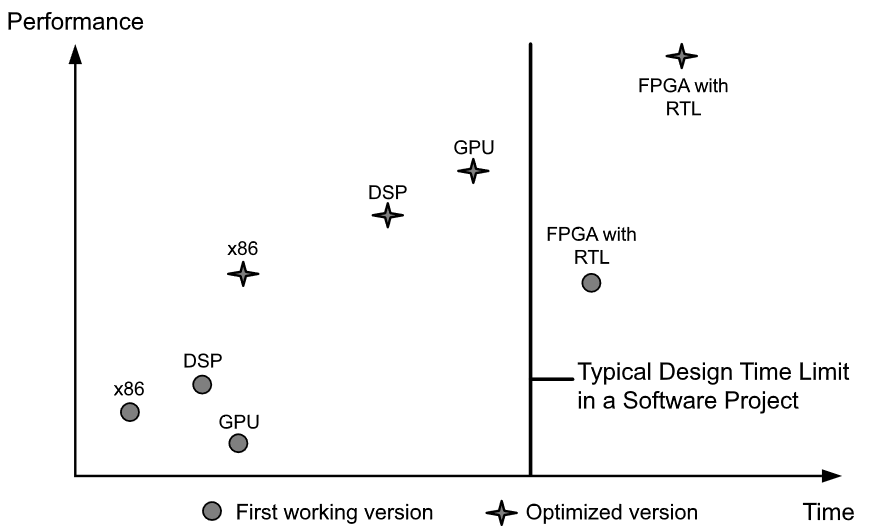
\includegraphics[width=0.7\textwidth]{fpgaRTL}
	\caption{Xilinx - Χρόνος σχεδιασμού \emph{vs. } Απόδοση εφαρμογής με RTL \cite{ug998}}
	\label{fig:fpgartl}
\end{figure}
\begin{figure}[H]
  	\centering
	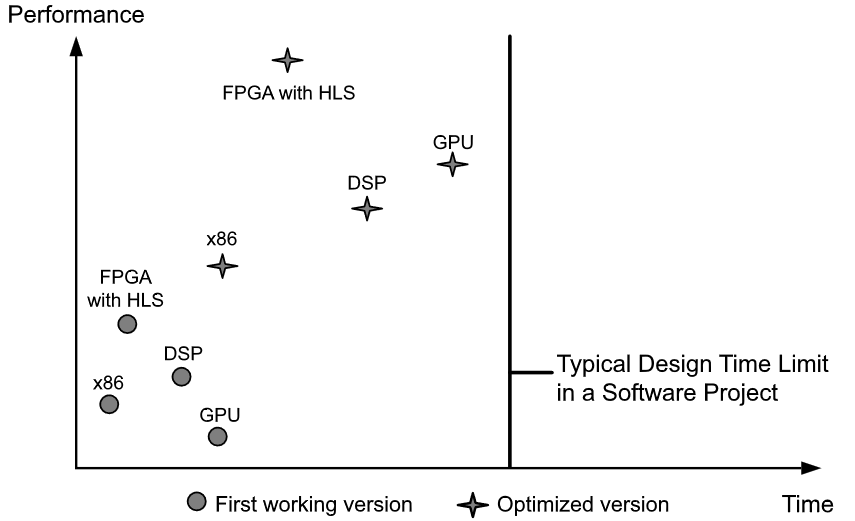
\includegraphics[width=0.7\textwidth]{fpgaHLS}
	\caption{Xilinx - Χρόνος σχεδιασμού \emph{vs. } Απόδοση εφαρμογής με HLS \cite{ug998}}
	\label{fig:fpgahls}
\end{figure}
\subsection{Γλώσσα προγραμματισμού VHDL}

Στον τρόπο προγραμματισμού που έχει επικρατήσει τις τελευταίες δύο δεκαετίες, ο σχεδιαστής υλικού παρέχει χειροκίνητα μία περιγραφή σε επίπεδο καταχωρητή, η οποία εφαρμόζεται στο υλικό μέσω HDL. Στη συνέχεια η περιγραφή RTL προσομοιώνεται με τη βοήθεια ενός προγράμματος που καλείται testbench. Εαν δεν υπάρχουν σφάλματα στη σχεδίαση δημιουργείται το \gls{net}. Στις περισσότερες περιπτώσεις, τα \gls{fpga} συνοδεύονται από μια πλατφόρμα λογισμικού του κατασκευαστή που χρησιμοποιείται για την παραγωγή του \gls{net}.

Η περιγραφή αυτή στη συνέχεια υλοποιείται στο \gls{fpga} μέσω μιας ειδικής διαδικασίας που καλείται place-and-route και τελικά παράγεται το δυαδικό αρχείο (bitstream) που απαιτείται για τον προγραμματισμό του. Το bitstream φορτώνεται στο \gls{fpga} μέσω διεπαφής JTAG ή εξωτερικής μνήμης.
\subsection{HLS}
\subsubsection{Επισκόπηση}

Ο κώδικας αναλύεται, περιορίζεται σε επίπεδο αρχιτεκτονικής και προγραμματίζεται ώστε να παραχθεί μια γλώσσα περιγραφής υλικού σε επίπεδο καταχωρητών, η οποία με τη σειρά της συνήθως συντίθεται σε επίπεδο πύλης με τη χρήση ενός λογικού εργαλείου σύνθεσης. Ο στόχος του \gls{hls} είναι να επιτρέψει στους σχεδιαστές υλικού να δημιουργήσουν και να ελέγξουν αποτελεσματικά το υλικό, παρέχοντάς του τον καλύτερο έλεγχο στη βελτιστοποίηση της αρχιτεκτονικής επιτρέποντας του παράλληλα να περιγράφει το σχέδιο σε υψηλότερο επίπεδο αφαίρεσης. Η επαλήθευση του RTL αποτελεί σημαντικό μέρος της διαδικασίας.
\begin{figure}[H]
  	\centering
	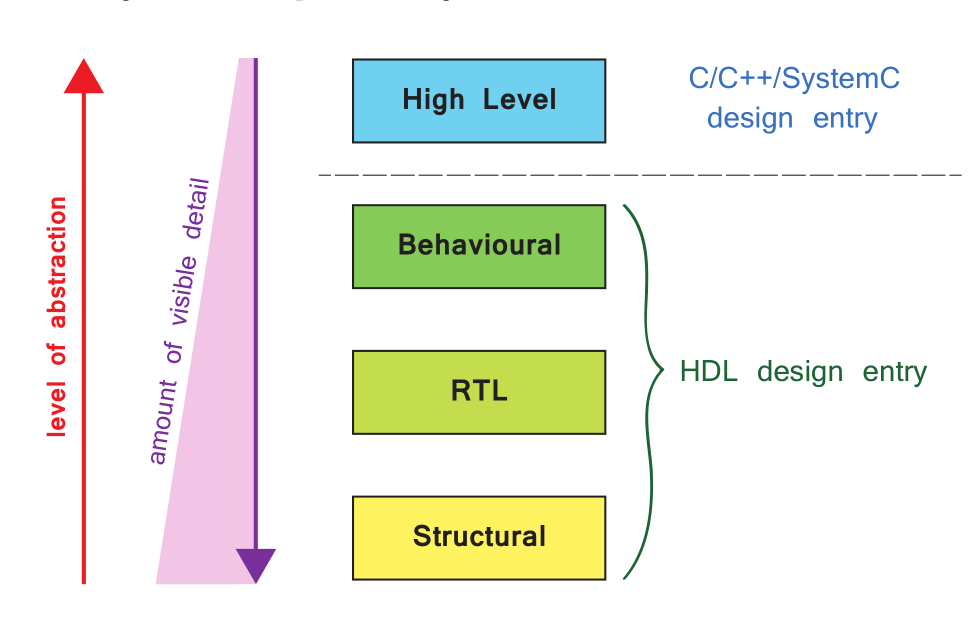
\includegraphics[width=0.5\textwidth]{abstraction}
	\caption{Επίπεδα αφαιρετικότητας σε σχεδιασμούς FPGA \cite{Crockett:2014:ZBE:2685817}}
	\label{fig:abstraction}
\end{figure}

Ενώ η λογική σύνθεση χρησιμοποιεί μια RTL περιγραφή του σχεδιασμού, η σύνθεση υψηλού επιπέδου λειτουργεί σε υψηλότερο επίπεδο αφαίρεσης, ξεκινώντας με μια αλγοριθμική περιγραφή σε μια γλώσσα υψηλού επιπέδου όπως η SystemC και η ANSI C/C ++. Ο σχεδιαστής αναπτύσσει τη λειτουργικότητα της μονάδας και το πρωτόκολλο διασύνδεσης και στη συνέχεια τα εργαλεία σύνθεσης υψηλού επιπέδου χειρίζονται την μικρο-αρχιτεκτονική και μετασχηματίζουν τον λειτουργικό κώδικα σε πλήρως χρονομετρημένες υλοποιήσεις RTL, δημιουργώντας αυτόματα λεπτομέρειες για τον κύκλο εκτέλεσης του υλικού.

Το ακόλουθο σχήμα (\ref{fig:hlsrtl}) διαθέτει τρεις άξονες που αναπαριστούν τις διαφορετικές όψεις του σχεδιασμού: συμπεριφορά (τί κάνει το υποκύκλωμα), δομή (πώς είναι δομημένο το κύκλωμα - \gls{net}) και γεωμετρία (πώς είναι δομημένο σε φυσικό επίπεδο το κύκλωμα - layout). Υπάρχουν επίσης πέντε ομόκεντροι κύκλοι που αντιπροσωπεύουν τα επίπεδα της αφαιρετικότητας: κυκλώματος, λογικής, RTL, αλγορίθμου και συστήματος.

\begin{figure}[H]
\centering
\subcaptionbox{RTL Design Flow}%
  [.45\linewidth]{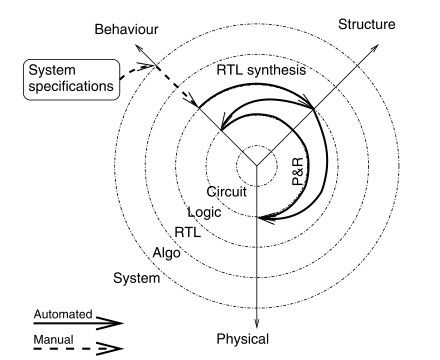
\includegraphics[width=0.45\textwidth]{RTLFlow}}
\subcaptionbox{\gls{hls} Design Flow}
  [.45\linewidth]{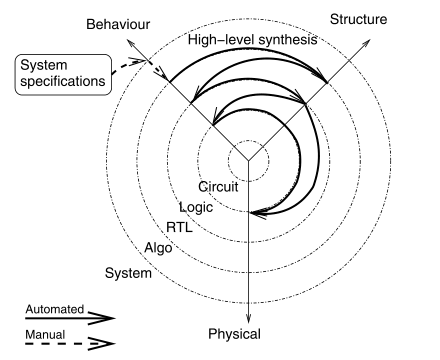
\includegraphics[width=0.45\textwidth]{HLSFlow}}
  \caption{High-level synthesis vs RTL στο Gasjki-Kuhn Y-chart \cite{Meeus2012}}
    \label{fig:hlsrtl}
\end{figure}

\subsubsection{Scheduling \& Binding}
Το HLS αποτελείται από δύο κύριες διεργασίες: scheduling και binding. Αυτές πραγματοποιούνται σε επαναληπτική βάση όπως φαίνεται στο επόμενο σχήμα καθώς η μία επηρεάζει την άλλη. Οι λειτουργίες των διεργασιών αυτών αναλύονται στη συνέχεια:
\begin{itemize}[label={},leftmargin=*]
	\item{\textbf{Scheduling}}

Είναι η διαδικασία της μετάφρασης των RTL δηλώσεων που μεταφράστηκαν από τον κώδικα C σε ένα σύνολο εντολών, καθένα με την αντίστοιχη διάρκεια εκφρασμένη σε κύκλους ρολογιού. Οι αποφάσεις που πραγματοποιούνται σε αυτό το στάδιο επηρεάζονται από τη συχνότητα του ρολογιού και την αβεβαιότητα του, την τεχνολογία της συσκευής που θα χρησιμοποιηθεί και τις ντιρεκτίβες που εφαρμόζονται από το χρήστη. \\

	\item{\textbf{Binding}}

Binding είναι η διαδικασία του συσχετισμού των προγραμματισμένων λειτουργιών με τους φυσικούς πόρους της συσκευής. Τα χαρακτηριστικά της λειτουργικότητας και του χρονισμού αυτών των πόρων μπορούν να επηρεάσουν τον προγραμματισμό των εργασιών, επομένως πληροφορίες σχετικές με το binding ανατροφοδοτούνται στη διαδικασία του scheduling.
\end{itemize}
\begin{figure}[H]
  	\centering
	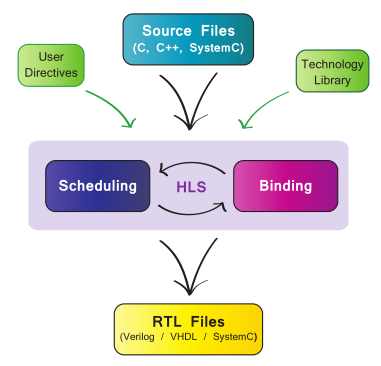
\includegraphics[width=0.6\textwidth]{scheduling}\\
	\caption{Ροή scheduling \& binding \cite{Crockett:2014:ZBE:2685817}}
	\label{fig:scheduling}
\end{figure}
\subsubsection{Design Flow}

Αναλυτικότερα, η πλήρης ροή σχεδιασμού με το HLS φαίνεται στο ακόλουθο σχήμα. Τα στάδια αυτά θα περιγραφούν στη συνέχεια.

\begin{figure}[H]
  	\centering
	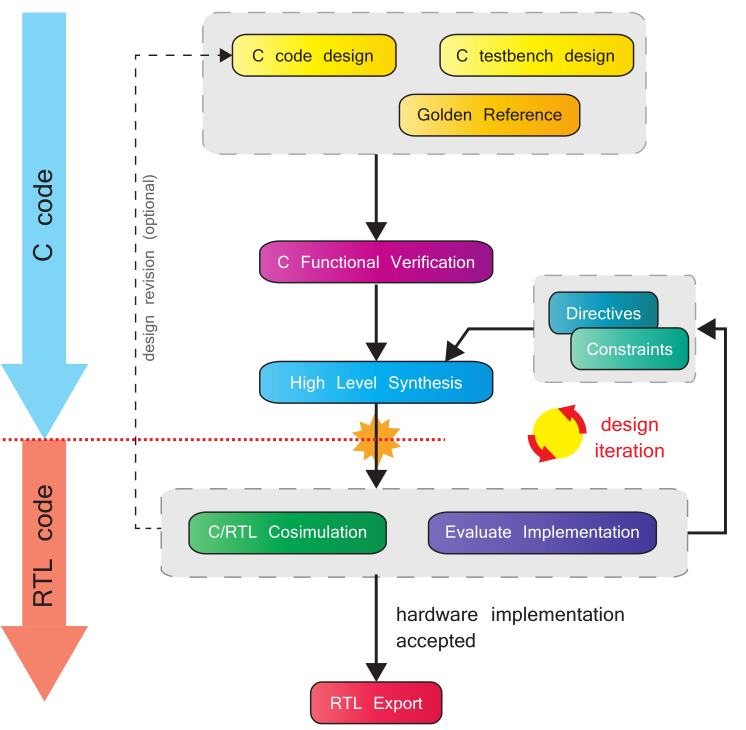
\includegraphics[width=0.6\textwidth]{hlsdflow}\\
	\caption{Ροή σχεδιασμού με HLS \cite{Crockett:2014:ZBE:2685817}}
	\label{fig:hlsdflow}
\end{figure}

\begin{itemize}[label={},leftmargin=*]
	\item{\textbf{Δεδομένα εισόδου στο HLS}}

	Τα πρωταρχικά δεδομένα εισόδου στο HLS είναι μία C/C++/systemC συνάρτηση καθώς και ένα αρχείο testbench το οποίο έχει αναπτυχθεί για να γίνει επαλήθευση της λειτουργίας της συνάρτησης. Το αρχείο αυτό περιέχει `golden data' τα οποία θα συγκριθούν με τα δεδομένα εξόδου της συνάρτησης. \\

	\item{\textbf{Λειτουργική επαλήθευση}}

	Αρχικά, είναι απαραίτητη η επαλήθευση της λειτουργική ακεραιότητας του κώδικα μας προτού παραχθεί ο κώδικας RTL με τη βοήθεια του testbench. \\

	\item{\textbf{Σύνθεση}}

	Επόμενο βήμα είναι η ίδια η σύνθεση υψηλού επιπέδου, η οποία περιλαμβάνει ανάλυση και επεξεργασία του κώδικα, των ντιρεκτίβων και περιορισμών ώστε να δημιουργηθεί μία περιγραφή RTL του υλικού.\\


	\item{\textbf{Προσομοίωση \& Αξιολόγηση}}

	Μετά τη δημιουργία του μοντέλου RTL, δοκιμάζεται η σωστή λειτουργία του (σε επίπεδο RTL) με τη βοήθεια του πρωτότυπου testbench. Εκτός της προσομοίωση πρέπει να γίνει όμως και μία αξιολόγηση των αποτελεσμάτων συγκριτικά με τις προδιαγραφές που είχαν οριστεί αρχικά.\\

	\item{\textbf{Εξαγωγή RTL}}

	Τελευταίο βήμα είναι η εξαγωγή του υλικού για τη χρήση του σε μεγαλύτερα συστήματα. Η μέθοδος της εξαγωγής σε IP είναι από τις πλέον κατάλληλες μορφές ώστε να εισαχθεί το υλικό στον IP Integrator, XPS ή System Generator.

\end{itemize}
\subsubsection{Βελτιστοποίηση}

Μεγάλη βαρύτητα πρέπει να δοθεί στις μετρήσεις και εκτιμήσεις απόδοσης του υλικού που σχεδιάστηκε. Πιο συγκεκριμένα πρέπει να εστιάσουμε:
\begin{itemize}
	\item Στους πόρους του FPGA που χρειάζονται για την υλοποίηση του σχεδίου μας και πως αυτοί συγκρίνονται με τους διαθέσιμους.
	\item Στη ρυθμοαπόδοση, δηλαδή σε τι ρυθμό μπορεί να επεξεργάζεται δεδομένα το υλικό.
	\item Στη μέγιστη συχνότητα ρολογιού που μπορεί να λειτουργεί το σχέδιο.
	\item Στο latency, δηλαδή πόσοι κύκλοι απαιτούνται για να παραχθεί η έξοδος.
	\item Στην κατανάλωση ισχύος του συστήματος και
	\item στις απαιτήσεις των απαιτούμενων διεπαφών. \\
\end{itemize}

Το Vivado HLS προσπαθεί από μόνο του να πετύχει το καλύτερο δυνατό σχεδιασμό RTL αν και τις περισσότερες φορές δίνει μεγαλύτερη έμφαση στην εξοικονόμηση πόρων θυσιάζοντας μέρος της απόδοσης του υλικού. Μας δίνεται όμως η δυνατότητα να πραγματοποιήσουμε βελτιστοποιήσεις κατά τη διάρκεια συγγραφής του κώδικα ώστε να επιτύχουμε την επιθυμητή απόδοση ή μία ισορροπία ανάμεσα στην απόδοση και την εξοικονόμηση πόρων. Στη συνέχεια αναλύονται οι βασικότερες μέθοδοι βελτιστοποίησης. \\
\begin{itemize}[label={},leftmargin=*]
\item{\textbf{Pipelining}}

Το pipeline είναι μία από τις πιο συνηθισμένες τεχνικές βελτίωσης του χρόνου καθυστέρησης διεργασιών. Διαιρώντας τα στάδια της επεξεργασίας σε πολλά μικρότερα τα οποία μπορούν να επεξεργαστούν διαφορετικά δεδομένα εισόδου ταυτόχρονα, επιτυγχάνεται η παραλληλοποίηση των διεργασιών. Σε όρους υλικού, αυτό επιτυγχάνεται με την εισαγωγή καταχωρητών ανάμεσα στα νέα μικρότερα στάδια, επιτρέποντας έτσι τη διατήρηση στη μνήμη των δειγμάτων εισόδου.
\begin{figure}[H]
		\centering
	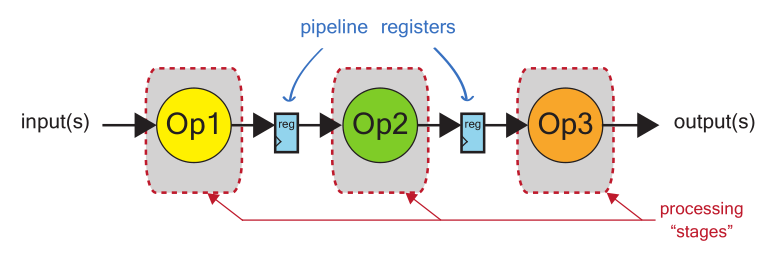
\includegraphics[width=0.7\textwidth]{pipeline}
	\caption{Διαμερισμός υπολογιστικών σταδίων σε μικρότερα μέσω pipelining \cite{Crockett:2014:ZBE:2685817}}
	\label{fig:hlsdflow}
\end{figure}

Με την τεχνική αυτή, η συνολική ρυθμοαπόδοση αυξάνεται σημαντικά και αρκετά συχνά παρατηρείται αύξηση στη μέγιστη συχνότητα λειτουργίας του υλικού. Αυτό συμβαίνει διότι τα τρία στάδια εντολών είναι πλέον ελεύθερα να επεξεργάζονται ταυτόχρονα συνεχόμενα δείγματα εισόδου όπως φαίνεται στο ακόλουθο σχήμα.

\begin{figure}[H]
	\centering
	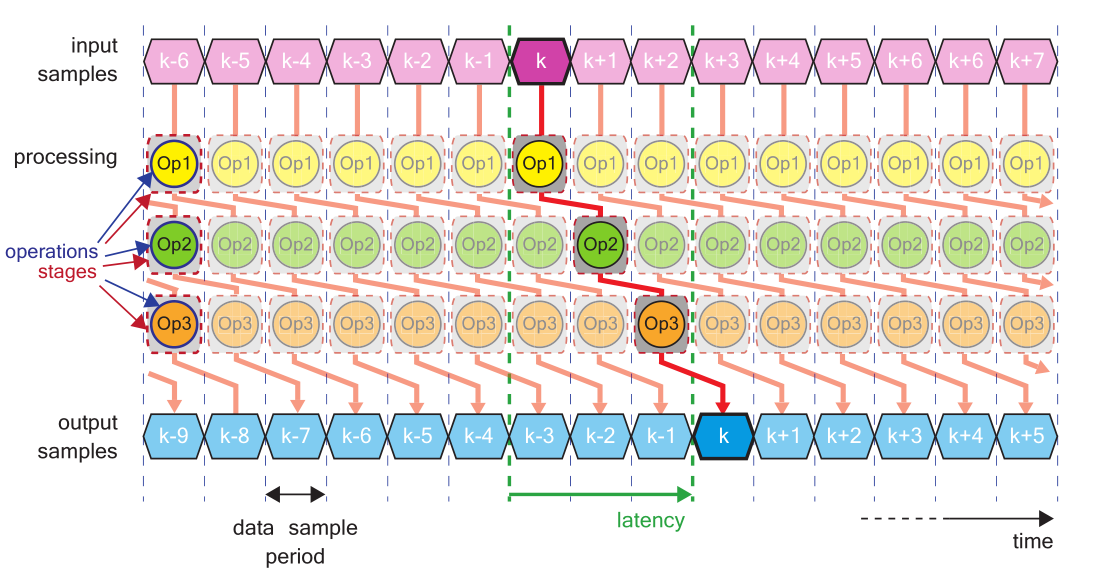
\includegraphics[width=\textwidth]{pipeline2}\\
	\caption{Latency \& ρυθμοαπόδοση μετά το pipelining \cite{Crockett:2014:ZBE:2685817}}
	\label{fig:hlsdflow}
\end{figure}

Πρέπει να δοθεί προσοχή σε ένα ακόμη μέγεθος, το Iteration Interval το οποίο εκφράζει τον αριθμό των κύκλων ανάμεσα στην είσοδο ενός νέου δείγματος εισόδου προς επεξεργασία. Χωρίς τη χρήση pipeline, το latency και το iteration interval μπορεί να ταυτίζοται καθώς το HLS βελτιστοποιεί το υλικό δίνοντας έμφαση στην εξοικονόμηση πόρων. Η στρατηγική χρήση pipeline μπορεί να τα μειώσει δραματικά. Όμως, η μείωση αυτή μπορεί να επιφέρει αυξημένη κατανάλωση πόρων επομένως χρειάζεται κάποιος συμβιβασμός. \\
\item{\textbf{Loop Unrolling}}

Οι βρόχοι χρησιμοποιούνται εκτεταμένα στον προγραμματισμό και αποτελούν μία φυσική μέθοδο για την αναπαράσταση διεργασιών που εκτελούνται επαναληπτικά. Με τη βοήθεια του Vivado HLS ο σχεδιαστής μπορεί να προτρέψει τους βρόχους να μετασχηματιστούν με διαφορετικούς τρόπους. Από προεπιλογή, οι βρόχοι είναι `rolled', μοιράζονται δηλαδή ένα ελάχιστο σετ υλικού το οποίο αποτελεί το κύριο σώμα του, επηρεάζοντας αρνητικά το συνολικό latency.

Οι βρόχοι επομένως μπορούν να ξετυλιχθούν (unrolled) κατά κάποιο βαθμό N ώστε να δημιουργηθούν N επαναλήψεις του υλικού επιτρέποντας κατ' αυτόν τον τρόπο την παράλληλη εκτέλεση των διεργασιών. Το μεγαλύτερο μειονέκτημα αυτής της μεθόδου είναι ότι μπορεί να οδηγήσει σε μεγάλα σχέδια υλικού. Και σε αυτή την περίπτωση πρέπει να γίνει κάποιος συμβιβασμός.
\noindent Για παράδειγμα ο ακόλουθος κώδικας,
\begin{lstlisting}[language=C++,belowskip=-1.2 \baselineskip]
for(int i = 0; i < X; i++) {
	#pragma HLS unroll factor=2
	  a[i] = b[i] + c[i];
}
\end{lstlisting}
\noindent μετασχηματίζεται στον:
\begin{lstlisting}[language=C++,belowskip=-1.2 \baselineskip]
for(int i = 0; i < X; i += 2) {
  	a[i] = b[i] + c[i];
  	if (i+1 >= X) break;
  	a[i+1] = b[i+1] + c[i+1];
}
\end{lstlisting}
\hfill \break
\item{\textbf{Dataflow}}

Η βελτιστοποίηση dataflow είναι παρόμοια με το pipeline που αναλύθηκε προηγουμένως αλλά στην πραγματικότητα εφαρμόζεται σε υψηλότερο επίπεδο στη σχεδιαστική ιεραρχία. Επιτρέπει στις συναρτήσεις του προγράμματος να επικαλύπτονται κατά τη λειτουργία, αυξάνοντας το συγχρονισμό της RTL υλοποίησης και της ρυθμοαπόδοσης. Για παράδειγμα, συναρτήσεις που προσπελαύνουν πίνακες πρέπει να ολοκληρώσουν όλες τις εντολές ανάγνωσης και εγγραφής σε αυτούς προτού ολοκληρωθεί η εκτέλεσή τους, αποτρέποντας την εκκίνηση λειτουργίας της επόμενης συνάρτησης. Η dataflow βελτιστοποίηση επιτρέπει επομένως, σε μία συνάρτηση ή βρόχο να ξεκινήσει τη λειτουργία της πριν την ολοκλήρωση της προηγούμενης.
\begin{figure}[H]
		\centering
	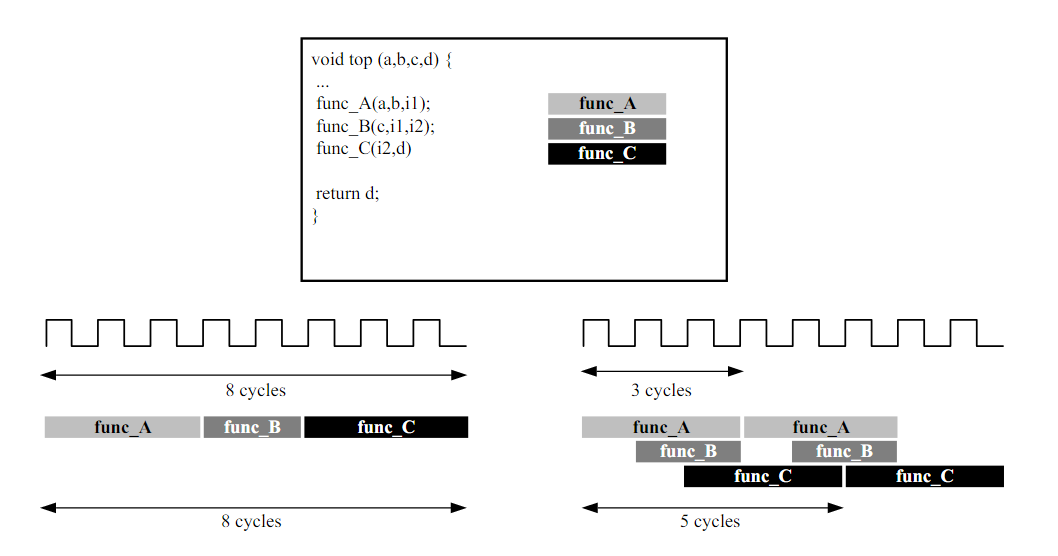
\includegraphics[width=0.7\textwidth]{dataflow}\\
	\caption{dataflow βελτιστοποίηση \cite{HLSPragmas}}
	\label{fig:hlsdflow}
\end{figure}
\item{\textbf{Array Optimizations}}

Στο Vivado HLS, οι πίνακες αντιπροσωπεύουν συνήθως αποθηκευτικό χώρο και για αυτό συντίθενται σε μνήμες. H μνήμη που ορίζεται κατά το HLS αντιστοιχίζεται σε φυσικούς πόρους του PL - BRAM/κατανεμημένη RAM - και είναι αναγκαίο να είναι γνωστό το μέγεθος της και πως αντιστοιχίζεται σε σχέση με τους διαθέσιμους πόρους του FPGA. Υπάρχει ένα σύνολο βελτιστοποιήσεων που μπορεί να εφαρμοστεί στους πίνακες κατα τη διάρκεια του σχεδιασμού.
\begin{itemize}
		\item \textbf{Resource}
		Ο σχεδιαστής μπορεί να επιλέξει σε τι μνήμη θα αντιστοιχίσει τον πίνακα.
		\item \textbf{Array Map}
		Με αυτή τη βελτιστοποίηση πολλοί μικροί πίνακες μπορούν να συνδυαστούν σε έναν μεγαλύτερο μειώνοντας έτσι τον απαιτούμενο αριθμό πόρων μνήμης.
		\item \textbf{Array Partition}
		Μπορεί να θεωρηθεί ως η αντίθετη τεχνική του Array Mapping καθώς επιτρέπει στο σχεδιαστή να διαιρέσει έναν πίνακα σε μικρότερους υποπίνακες ώστε να αυξήσει το ρυθμό με τον οποίο πραγματοποιούνται μεταφορές δεδομένων από/προς τη μνήμη (πχ 2-port BRAM).
		\item \textbf{Array Reshape}
		Η ντιρεκτίβα αυτή επιτρέπει έναν πίνακα με μεγάλο αριθμό στοιχείων μικρού μήκους, να μετασχηματιστεί σε έναν πίνακα με λιγότερες αλλά μεγαλύτερες λέξεις μειώνοντας έτσι το συνολικό αριθμό προσπέλασης της μνήμης.
		\item \textbf{Stream}
		Με την εντολή Stream, ο πίνακας αντιστοιχίζεται σε δομές FIFO αντί RAM.
	\end{itemize}
\end{itemize}
\subsubsection{Περιορισμοί HLS}

Η πλατφόρμα Vivado HLS ενώ υποστηρίζει ένα μεγάλο εύρος της γλώσσας προγραμματισμού C, ένα σύνολο constructs της δεν είναι συνθέσιμα ή μπορούν να οδηγήσουν σε σφάλματα κατά τη διάρκεια της σχεδιαστικής ροής \cite{ug902}. Για να είναι ο κώδικας συνθέσιμος πρέπει:
\begin{itemize}
	\item{Να περιέχει το σύνολο της λειτουργικότητας της σχεδίασης}
	\item{Να μην βασίζεται σε κλήσεις του συστήματος για την πραγματοποίηση λειτουργιών}
	\item{Οι δομές μνήμης να είναι στατικές και όχι δυναμικές} \\
\end{itemize}

Οι κλήσεις συστήματος δεν είναι συνθέσιμες καθώς είναι ενέργειες που σχετίζονται με την εκτέλεση εργασιών βασισμένων στο λειτουργικό σύστημα στο οποίο τρέχει ο κώδικας. Το Vivado HLS αγνοεί αυτό το είδος εντολών που δεν έχουν καμία επίδραση στην εκτέλεση του προγράμματος. Αν η χρήση τους όμως είναι αναγκαία για την πραγματοποίηση αποσφαλμάτωσης, τότε με τη βοήθεια του \textbf{macro \_\_SYNTHESIS\_\_} το Vivado HLS εξαίρει το συγκεκριμένο κομμάτι κώδικα. Για παράδειγμα:
\begin{lstlisting}[language=C++,belowskip=-1.2 \baselineskip]
#ifndef __SYNTHESIS__
ofstream myfile;
myfile.open ("example.txt");
myfile << "Hello World!\n";
myfile.close();
#endif
\end{lstlisting}

Οποιαδήποτε εντολή που διαχειρίζεται την κατανομή μνήμης, όπως για παράδειγμα οι \textbf{malloc()}, \textbf{alloc()} και \textbf{free()}, χρησιμοποιεί πόρους που υπάρχουν στη μνήμη του συστήματος που δεσμεύονται ή ελευθερώνονται κατά τη διάρκεια της εκτέλεσης. Τέτοιες εντολές πρέπει να αφαιρούνται από το σχεδισμό πριν τη σύνθεση και οι δυναμικές δομές να μετατραπούν σε στατικές με γνωστά όρια.
